	
\documentclass[review]{elsarticle}
\usepackage{hyperref,lineno}
\usepackage{xcolor}
\usepackage[utf8]{inputenc}
\modulolinenumbers[5]

%\newcommand{\memo}[2]{\textcolor{#1}{#2}}
%\newcommand{\maria}[1]{\memo{red}{#1\\}}
%\newcommand{\revise}[1]{\memo{blue}{#1\\}}

\journal{Journal of Archaeological Science}


\bibliographystyle{model2-names.bst}\biboptions{authoryear}


\begin{document}

\begin{frontmatter}

\title{Identifying social learning between Roman amphorae workshops through morphometric similarity}


\author[bscadress,ceipacadress]{Maria Coto-Sarmiento\corref{mycorrespondingauthor}}
\cortext[mycorrespondingauthor]{Corresponding author}
\ead{maria.coto@bsc.es}


\author[edadress]{Xavier Rubio-Campillo}
\author[ceipacadress]{Jos\'e Remesal}


\address[bscadress]{Barcelona Supercomputing Center (BSC), Jordi Girona 29, Office 3A, Nexus II Building, 08034, Barcelona, Spain}
\address[edadress]{School of History, Classic \& Archaeology, Room OOM.33, William Robertson Wing, Old Medical School, Teviot Place, University of Edinburgh, UK}
\address[ceipacadress]{CEIPAC, Department of Prehistory and Archaeology, Montalegre, 6-8, 08001, University of Barcelona, Barcelona, Spain}

\begin{abstract}

The aim of this study is to identify dynamics of social learning between amphorae workshops during the the Roman Empire. The Baetica province developed a massive infrastructure of olive oil production that supplied the Western provinces of Rome for almost 300 years. The olive oil produced in this area was shipped through maritime and riverine transport networks in a standardized amphoric shape made in several workshops spread around the region. These workshops have generated a large amount of evidence but it is still difficult to understand through archaeological proxies how the production of amphorae was organized.

We apply here an evolutionary framework to find links between workshops through the morphometric similarities of the amphorae they produced. The suggested approach identifies how individual potters acquired and transmitted technical skills by exploring small yet statistical significant differences in the amphorae made in 5 different workshops. Multivariate methods are used to cluster a variety of amphorae based on morphometric measurements and the outcome shows that the analysis is useful even when a high degree of standardization exists, such as was the case for Roman amphorae (i.e. Dressel 20).

Results suggest that morphometric similarity is inversely correlated with spatial distance between workshops. This pattern suggests that pottery-making techniques were transmitted through oblique transmission with little or no movement of potters between distant workshops. The conclusion is that morphometric similarity may be an effective proxy to identify social learning dynamics even amongst workshops producing exactly the same amphoric type. 

\end{abstract}


\begin{keyword}
Roman Empire; amphora workshops; Dressel 20; social learning; cultural evolution
\end{keyword}

\end{frontmatter}

\linenumbers

\section{Introduction}

The archaeological record is useful to identify the mechanisms by which humans learn from each other~\citep{richerson2005not,eerkens_jelmer_cultural_2007}. The analysis of archaeological proxies able to capture variability can help us find traces of the social learning dynamics of the techniques used to made them~\citep{shennan_ceramic_2001,eerkens_jelmer_cultural_2005, gandon_copying_2014}. This approach has been successfully applied to the material culture generated by small-scale societies, but it has seldom been applied to large-scale standardized productions~\citep{shennan_isolation-by-distance_2015}.

This paper explores the social dynamics of specialized production in the Roman Empire. We focus here on analysing large-scale production of a single amphoric type (Dressel 20) in a specific area. An evolutionary framework is used to identify social learning dynamics between pottery-makers \citep{shennan_evolution_2008,mesoudi_cultural_2015}. 

Specifically, pottery making is learned through a variety of cultural transmission mechanisms depending on the organization of the community that made them~\citep{neff1992ceramics,shennan_genes_2002,bowser_learning_2008,hosfield_modes_2009}. For example, vertical transmission is a mode of transmission where learning is transmitted from parents to offspring (similar to biological transmission); oblique transmission sees a master teaching a younger generation of disciples, whereas in horizontal transmission individuals of the same generation transmit their knowledge to other individuals of the same generation (i.e. workers of different workshops)~\citep{cavalli-sforza_cultural_1981, acerbi_cultural_2006}.

All these methods require communication and for this reason the techniques to make artefacts such as pots and amphorae should vary across geographical distance~\citep{bjorklund_effect_2010,shennan_isolation-by-distance_2015, van_strien_isolation-by-distance_2015}. If vertical or oblique transmission are predominant then material culture should be similar in nearby groups with high intensities of interaction \citep{hart_effects_2012}. The underlying consequence is that it should be possible to identify the degree of interaction between workshops by quantifying similarity amongst the amphorae they produced; if apprentices moved between distant workshops then no differences would be found on this proxy while oblique transmission would be revealed by distant workshops exhibiting less similarity.

These hypotheses on archaeological proxies of social learning have been tested elsewhere~\citep{roux_standardization_2015} and it has been shown that handmade pottery can be a good indicator of the different social learning mechanisms involved on the process~\citep{steele_james_ceramic_2010,neiman_stylistic_1995, shennan_ceramic_2001}. However, cultural transmission on standardized productions such as the ones found during the Roman Empire has not been explored at the same level~\citep{bevan_mediterranean_2014}.

The work we present here identifies learning processes of amphorae making in the case of the massive olive oil production organised during the Roman Empire. Olive oil was one of the most important products of the Classical Mediterranean world as it was used in almost all aspects of daily life including cooking, lightning and hygiene \citep{mattingly_d.j._oil_1988}. The Baetica province (currently Andalusia, southern Spain) developed a massive infrastructure of olive oil production to face the demands of the Roman Empire. The product was shipped in large amounts of amphorae to distant provinces all along the Western provinces and specially to the city of Rome and the thousands of military garrisons deployed along the provinces in the border such as Britannia~\citep{monfort_britannia_1998,funari_economic_2005} and Germania \citep{remesal_annona_1986}. 

Baetica was an important olive oil production and distribution centre for almost three centuries \citep{millet_anforas_1998, rodriguez_baetican_1998,chic2005comercio,rodriguez_economioleicola_1977}. The province had a strong connectivity through riverine transport that allowed inland producers to ship their products towards the trade networks through the Mediterranean and the Atlantic \citep{garcia_vargas_enrique_formal_2010}. The production of amphora shipping Baetican olive oil exhibits a sudden exponential increase as over a hundred of workshops were created to meet the volume of olive oil being produced. These workshops were located along the Guadalquivir river and its tributaries. The majority of amphorae produced in this area are classified as Dressel 20 type divided into a variety of subclasses \citep{martin-kilcher_romischen_1994,berni_millet_epigrafianforica_2008}.

Despite the abundance of Dressel 20 across thousands of archaeological sites, we still do not know how its production was organized. This challenge is common for all large-scale productions during the Roman Empire due to the lack of written records discussing the topic and the difficulties of identifying adequate archaeological proxies that give clues on the process. Several studies have analysed amphorae using a diversity of approaches, from chemical analyses to large-scale distribution \citep{isaksen_network_2006,brughmans_roman_2016,coto-sarmiento_maria_bayesian_????}. However, the structure of social learning that transmitted knowledge on how amphorae were made is still poorly understood. Were these workshops run by families or groups of owners without kinship? Did apprentices worked in the same workshop where they were trained? Did potters work in more than one workshop? Were changes in production decided by workshops or by external actors? All these questions are linked to the social learning processes that took place in the workshops. Additionally, archaeological record shows this specialized production was highly organized and homogeneous both in terms of products and processes. As a consequence, amphorae made in different workshops do not exhibit a large degree of variations and they look identical: the same type of amphorae was produced over 300 years while similar stamps and information was recorded on them \citep{remesal_anforas_2004}.

We use here an evolutionary framework designed to improve our understanding of these large-scale production dynamics. If the system was mainly driven by oblique transmission mechanisms then no potters would be moving to distant workshops. As a consequence, amphorae produced in nearby workshops might share more similar traits than with the rest of the production. On the other hand, if horizontal dynamics were common then this correlation with spatial coordinates should not be present as workers would share their methods across space.

The paper is structured as follows: the next section introduces the dataset and the methods used to analyse it. Section three presents the results while the last part discusses the outcomes and highlights the main conclusions of the work. 

\section{Material and methods}

\subsection{Workshops}

Our sample comprised 413 Dressel 20 amphorae collected from the five Dressel 20 workshops most intensively excavated during recent decades: Malpica, Cerro del Belén (hereafter, Belén)~\citep{diaz_trujillo_excavacion_1992}, Parlamento \citep{garcia_vargas_anforas_2000}, Villaseca~\citep{garcia_vargas_enrique_excavacion_????} and Las Delicias~\citep{fernandez_excavacion_2001,_atelier_2014} (see their location in Figure \ref{romanworkshop}).

\begin{figure}[htp]
	\centering
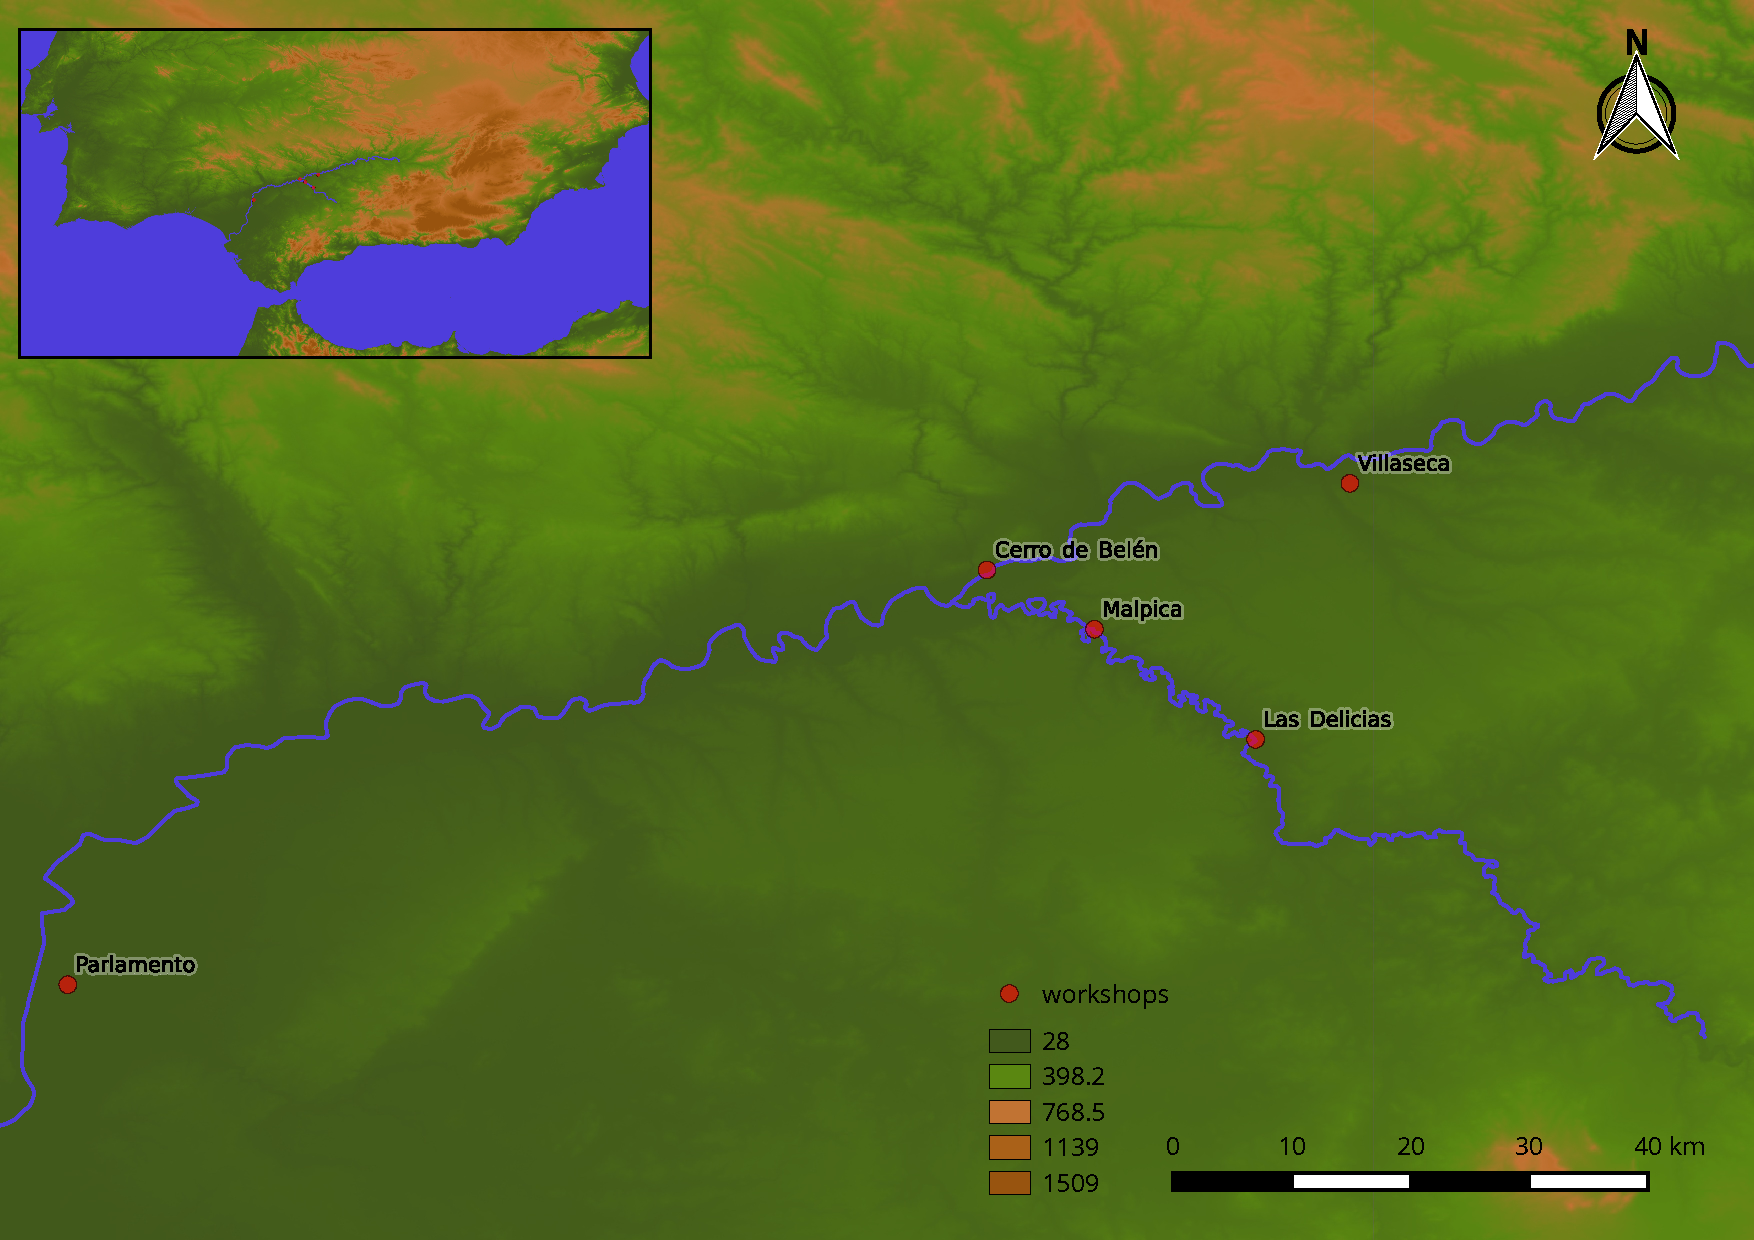
\includegraphics[width=\linewidth]{figs/romanworkshop}
\caption{The Baetica province during the Roman Empire. The location of the analysed workshops shows how Dressel 20 workshops were mostly distributed along the rivers Gualdalquivir and Genil}
\label{romanworkshop}
\end{figure} 

The sample was roughly uniformly distributed as the 5 workshops provided a similar sample size (80-100 samples). These workshops were distributed in a diversity of locations therefore spatial dynamics could be potentially identified. All of them had a long time span of production; however, temporal variation was limited as the Dressel 20 type remained almost unchanged over three centuries~\citep{berni_dressel_2016}. We analysed Dressel 20 of the three most abundant variants in our dataset spanning approximately three centuries (Dressel C, Dressel D, Dressel E)~\citep{martin-kilcher_romischen_1994,berni_millet_epigrafianforica_2008}. All the variants were found in the 5 workshops and, consequently, no intrinsic bias was generated by them. 

\subsection{Spatial Distance}

The approach required us to compute a pairwise matrix of spatial distances between workshops. All these workshops were located near a river as the amphorae were shipped by boat after being made and filled with olive oil. Given the relevance of riverine transport, it was decided that the best proxy for spatial distance between workshops was the one observed following the river course, as summarized in Table~\ref{table:distances}.

\begin{table}[htp]
\centering

\begin{tabular}{lccccc}
\hline

\textbf{Workshops} & Malpica & Belén & Villaseca & Las Delicias & Parlamento \\ \hline
Malpica & - & 11 & 50 & 17 & 108 \\
Belén & 11 & - & 33 & 29 & 98 \\
Villaseca & 50 & 33 & - & 67 & 133 \\
Las Delicias & 17 & 29 & 67 & - & 126 \\
Parlamento & 108 & 98 & 133 & 126 & - \\
\hline
\end{tabular}
\caption{River distance matrix between workshops (in km.)}
\label{table:distances}
\end{table}

\subsection{Measurements}

Eight different measurements were taken from each amphora. The metrics were focused on the rim sherds as this section was typically the best preserved in most archaeological contexts~\citep{berni_millet_epigrafianforica_2008}. Other interesting proxies such as handles and bases were found in lesser quantities and for this reason they would be less appropriate for quantitative approaches due to low sample size. The measurements used in this study are summarized in Figure~\ref{mesures}; they were divided into exterior diameter, inside diameter, rim height, rim width, shape width, rim inside height, rim width 2 and protruding rim.

\begin{figure}[htp]
	\centering
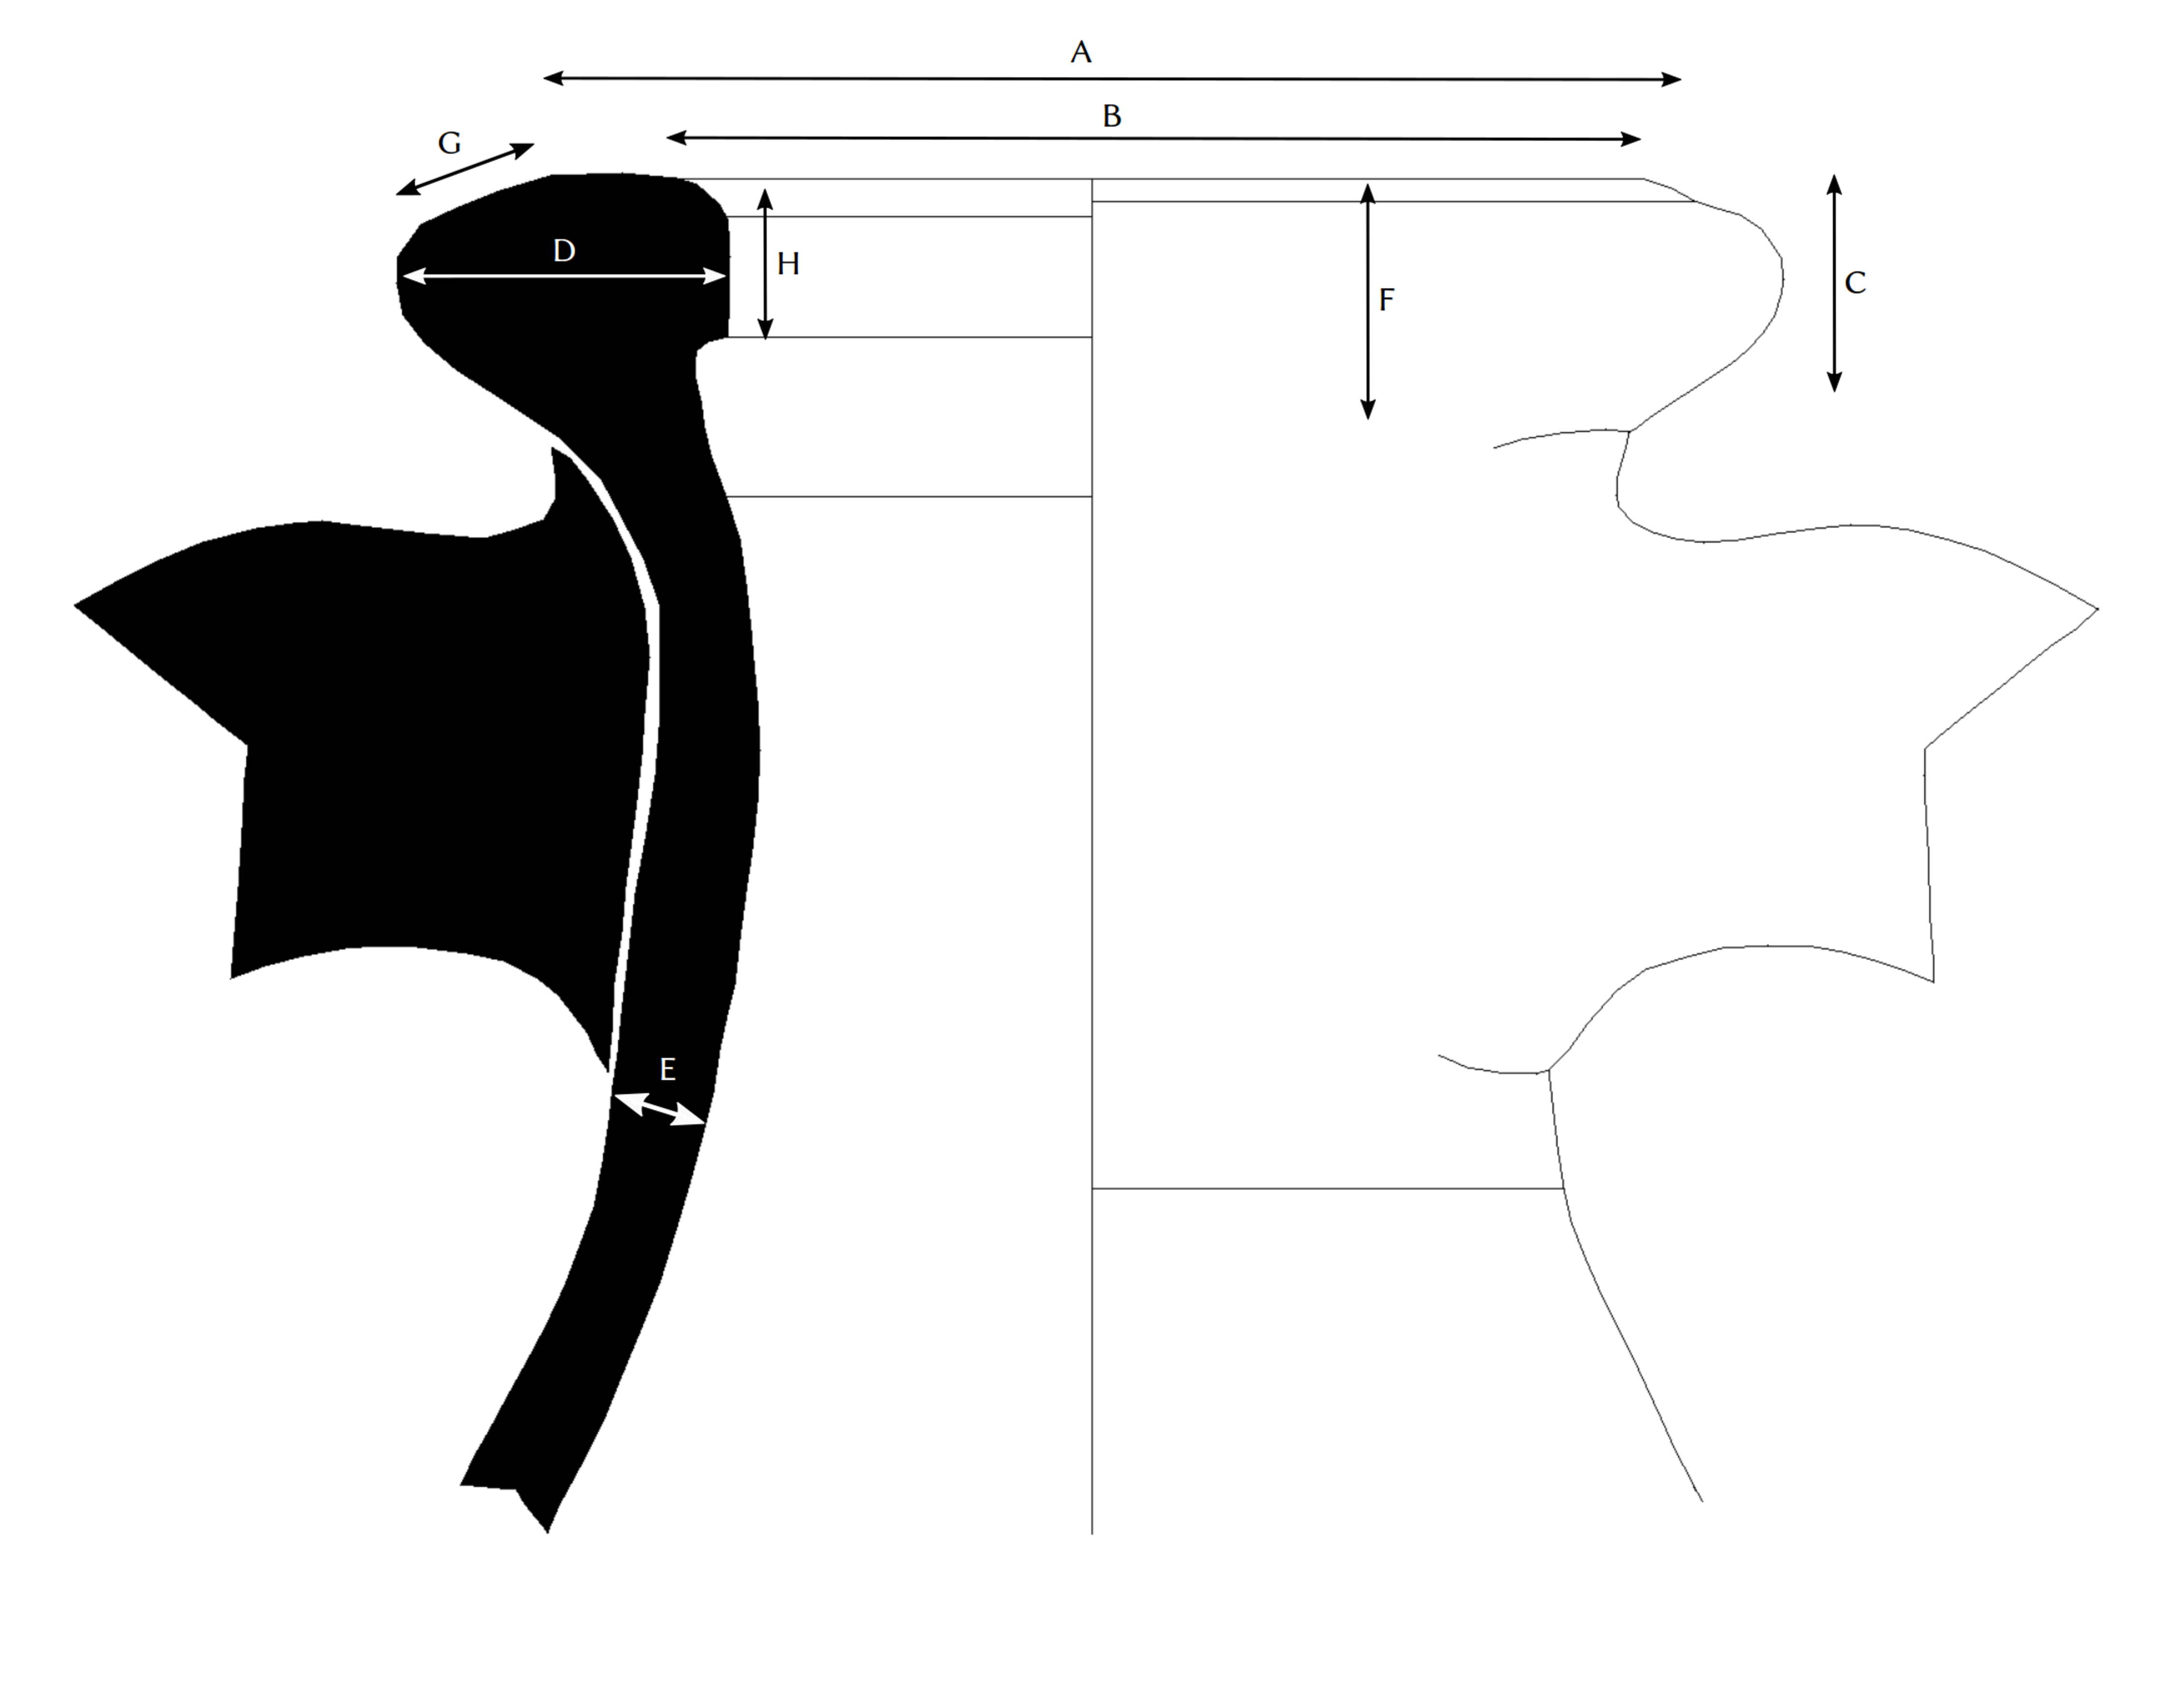
\includegraphics[width=\linewidth]{figs/mesures.pdf}
\caption{The 8 morphometric measurements taken for all amphorae. A: External diameter. B: Inside diameter. C: Rim height. D: Rim width. E: Shape width. F: Rim inside height. G: Rim width 2. H: Protruding rim.}
\label{mesures}
\end{figure} 

\subsection{Exploratory Data Analysis}

Principal Component Analysis (PCA) was used to explore the variation of the measurements over the different workshops \citep{jolliffe_principal_2002}. PCA is a common method in archaeology in scenarios studying within-sample variation \citep{shennan_quantifying_1997, li_crossbows_2014, schillinger_differences_2016}. The method allowed us to visualize the dataset by focusing on a small number of Principal Components (PCs) while retaining the variation required to identify differences between workshops. 

\subsection{Morphometric similarity} 

Exploratory Data Analysis was followed by the measurement of pairwise dissimilarity between the amphorae made in different workshops. The approach presented here is based on the following idea: if the amphorae made in two workshops are difficult to distinguish then the workshops are making more similar artefacts. On the other hand, if the probability of distinguishing the production place of the combined dataset is high then there are remarkable morphometric differences between the artefacts made in different workshops. This goal was achieved by 1) train a clustering algorithm with the entire dataset, 2) use the trained model to predict the producer's workshop and 3) calculate the confusion matrix between the workshops.

The clustering method used in the analysis was Linear Discriminant Analysis (LDA). The entire dataset was used both for the training and prediction steps as we were interested on identifying under what extent workshop attribution could be predicted relying exclusively on morphometric measures. A Confusion Matrix was then computed as the index of morphometric distance between amphorae of different workshops. The Confusion Matrix computes this quantity as the number of misclassifications between each pair of groups in the dataset (i.e. the workshops). This method has already been used in similar scenarios aiming at identifying differences in artefact production \citep{thorpe_distribution_1984,i_martin_alisis_1998,charlton_investigating_2012}. If the amphorae made in two workshops were easily confused then their average measures must be similar; on the other hand, if the rate of misclassification between two workshops is very low then the amphorae made in these locations are distinctively different.

The diagonal of the confusion matrix (i.e. correct classifications) was removed and the number of confusions per each workshop was then divided by the total sample size. This value defined the percentage of errors from a given workshops related to the rest of the sample. The outcome was finally normalized to generate a pairwise distance matrix of morphometric measurements.

\subsection{Dissimilarity correlation}

The last step of this method was the comparison of the morphometric and spatial distance matrices. A significant correlation between these dissimilarity matrices would suggest isolation-by-distance typically found if oblique transmission was the main social learning mechanism.

The evaluation of these two distance matrices (morphometric distance and spatial distance) was computed using a Mantel test. Mantel test evaluates the degree of pairwise correlation between two matrices and has been particularly useful in archaeology to explore the spatial dimension of cultural change \citep{mantel_detection_1967, diniz-filho_mantel_2013, crema_culture_2014}.  

\section{Results}

\subsection{Principal Component Analysis}

The loadings for the two main Principal Components of the dataset are listed in Table~\ref{table:pca}.

\begin{table}[htp]
\centering
\begin{tabular}{lcccccccc}
\hline
Variables & PC1 & PC2 \\ \hline
Exterior diameter & 0.877 & 0.312 \\
Inside diameter & 0.404 & -0.887 \\
Rim height & - & - \\
Rim width & 0.149 & 0.119 \\
Shape width & - & - \\
Rim inside & - & - \\
Rim width 2 & 0.133 & 0.142 \\
Protruding rim & -0.159 & -0.272 \\
\hline
\end{tabular}
\caption{Two main Principal Components. Diameter values and the protruding rim seem to capture the majority of variation.}
\label{table:pca}
\end{table}

An exploratory visualization for these two main Principal Components can be seen in Figure \ref{pca}. The plot suggests that each workshop exhibits slightly different dynamics for PC1 while PC2 is distinctively different for the two most distant sites (Villaseca and Parlamento). Additionally, the first PC also tends to display more similar values for amphorae made in nearby workshops such as Belén and Malpica. The exploratory analysis was also performed for different Dressel 20 types in order to observe possible patterns linked to their chronology. A similar pattern is observed in Figure \ref{dressel}. The result suggests a noticeable difference between Dressel C and Dressel D and E but barely perceptible between Dressel D and E.

\begin{figure}[htp]
	\centering
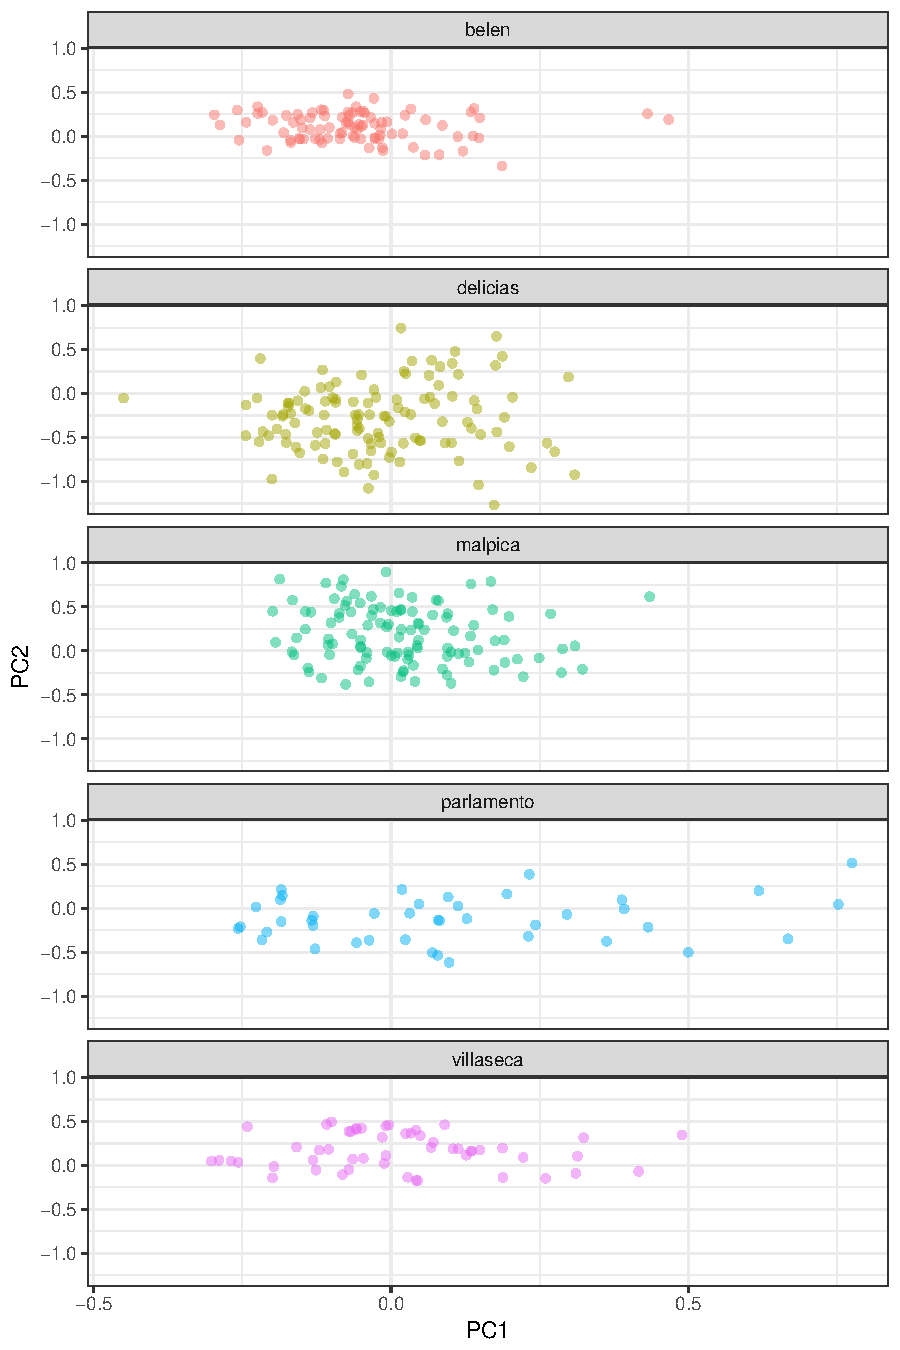
\includegraphics[width=\linewidth]{figs/pca}
\caption{Scatter and density plot for the First and Second PCs. Sample is split by workshop}
\label{pca}
\end{figure} 


\begin{figure}[htp]
	\centering
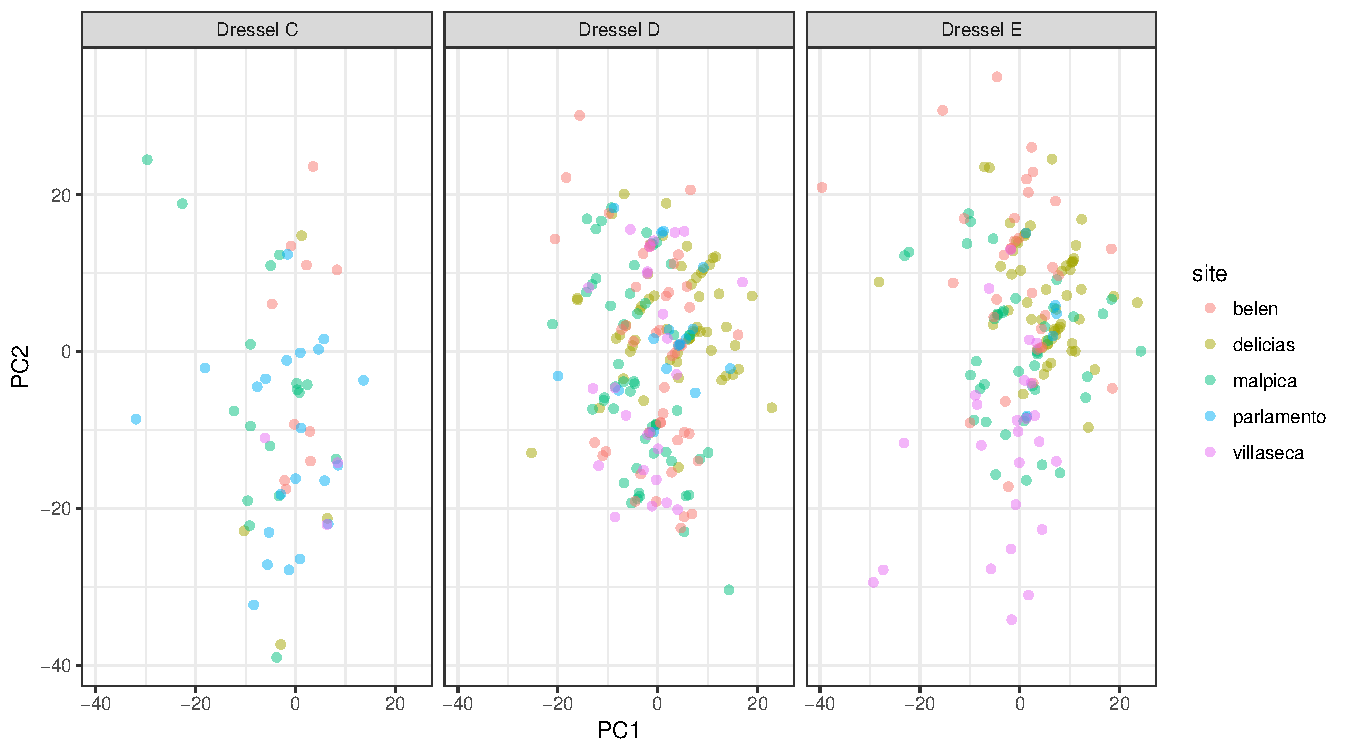
\includegraphics[width=\linewidth]{figs/dresseltypes}
\caption{Scatter plot for the First and Second PCs. Sample is divided by Dressel 20 types}
\label{dressel}
\end{figure} 


\subsection{Linear Discriminant Analysis}

LDA's prediction generated an overall accuracy of 56.6\%. It is worth mentioning that we are not as interested on the overall accuracy of the clustering algorithm as we are on the distribution of these errors across workshops. This distribution can be seen in the Confusion Matrix of Table~\ref{table:confusion}. Each row of the matrix represents the predicted class whereas each column represents the real class. It can be observed that the most distant workshop (Parlamento) can be more easily predicted while the classification for the rest of the sample is less effective.

\begin{table}[htp]
\begin{tabular}{lccccc}
\hline
      & Belén & Delicias & Malpica & Parlamento & Villaseca\\ \hline
Belén & 48 & 11 & 16 & 4 & 6 \\
Delicias & 10 & 81 & 24 & 8 & 0 \\
Malpica & 12 & 12 & 49 & 1 & 6 \\
Parlamento & 6 & 10 & 9 & 25 & 10 \\
Villaseca & 12 & 5 & 13 & 4 & 31 \\
\hline

\end{tabular}
\caption{Confusion Matrix of errors in predicted classifications between workshops. The sample analysed gave an accuracy percentage of 56.6\% with p-value $<$0.01. }
\label{table:confusion}
\end{table}

A temptative glance to these results suggests that workshops with lesser spatial distance such as Malpica, Belén and Las Delicias made amphorae that are more difficult to distinguish due to their similarity. By contrast, workshops as Parlamento shows a higher degree of misclassification that correlated with a higher spatial distance. 

\subsection{Mantel correlation test}

The Mantel test applied to morphometric and spatial similarity generated a correlation of $0.51$ with p-value under $0.01$. The analysis shows that morphometric distance of the amphorae are strongly correlated with the spatial distance of workshops. Closer workshops tend to be generate more similar amphorae than distant workshops. For example, Belén and Malpica are located at nearby positions and the morphometric distance seems more similar whereas Parlamento displays significant differences with the rest of workshops. Thus, the results suggest that the variability on the making-techniques processes are related to spatial distance.

\section{Discussion and Concluding remarks}

Similarity on the making techniques processes amongst workshops shows an inverse correlation with spatial distance. This phenomena can be explained by isolation-by-distance as mobility between workshops was limited. The similarity of morphometric traits of the analysed sample decreases with spatial distance and as a result amphorae made in nearby workshops were more similar than amphorae made in distant workshops because contact between workers was less frequent. 

Horizontal transmission or high mobility do not seem to match with the results of the analysis. Scenarios with frequent contact between potters or workers moving from workshop to workshop would have generated larger homogeneity in the metrics. In addition, the morphological variability detected in different workshops also suggest that making-techniques were typically shared across workshops. No distinctive variation has been detected in the analysis and this outcome suggests that potters reproduced the same model of amphorae with a very slow rate of variation.
  
Oblique transmission could be the main social learning mechanism to explain the variability between these workshops. The equilibrium of this dynamic for a long timespan (over three centuries) can be interpreted as a high-fidelity social learning mechanism transmitted within each one of the workshops \citep{schillinger_copying_2016}. The disciples could have worked at the same workshop where they were trained and as a consequence individuals would have copied the model of amphora made by the previous generation within the same workshop. Small random errors would have been transmitted and amplified across the period and each workshop would have produced slighly different amphora assemblage. The large degree of standardization would have minimized these differences but our framework is still able to identify them.

It is worth mentioning that the diversity of social learning processes involved on such a complex process is always high. The transmission of technical skills during apprenticeship (master to disciples) and their limited mobility does not imply that horizontal transmission did not exist. The process initially led by masters within the same workshop could be complemented by periods of high mobility of the workers linked to peaks of production.

To conclude, the method presented here provides a framework to identify social learning mechanisms using artefacts made in different sites. The method has proven valuable even in the case of the highly standardized amphoric production of the Roman Empire. The suggested method could also offer a good comparison with other analytical methods such as archaeometry; we believe that a framework integrating and comparing multiple sources of evidence could be extremely effective on the process of characterizing production sites and places of consumption. Our analysis provides a useful guideline for the exploration of the social learning processes connected with amphora production in the Roman Empire. Hence, the results have lightened to understand the link between social learning and archaeological evidence in a diversity of scenarios. 
 

\section{Acknowledgments}

The research was funded by the EPNet project (European Research Council Advanced Grant - 340828). We are grateful to Enrique Garc\'ia Vargas, Simon Carrignon, Juan Moros for their useful comments and the two anonymous reviewers and editor for helpful suggestions and constructive comments on previous versions of the paper. The Museum of \'Ecija (Antonio Fern\'andez Ugalde), Museum of Palma del R\'io (Reyes Lopera and Emilio Navarro), Museum of C\'ordoba and Museum of Seville for kindly allowing us access to their information. Data were collected, performed and analysed in R version 3.2.4. statistical language and implemented with the packages MASS, vegan and ggplot2 \citep{ripley_package_2013,oksanen_vegan_2007,ggplot2:_2016}. Map was done by QGIS 2.18.15 'Las Palmas' with SRTM data Version 4.1 from CIAT-CSI SRTM website (http://srtm.csi.cgiar.org) \citep{SRTM}. 

Source code and datasets are freely available and can be downloaded from https://github.com/Mcotsar/LearningBaetica.  

\section*{References}

\bibliography{mybibfile}

\end{document}

\cite
